\chapter{Mesh Generation}
%

%%%%%%%%%%%%%%%%%%%%%%%%%%%%%%%%%%%%%%%%%%%%%%%
%%%%%%%%%%%%%%%%%%%%%%%%%%%%%%%%%%%%%%%%%%%%%%%
\section{Hexahedral and Hex-Dominant Meshing}
\label{Hexahedral and Hex-Dominant Meshing}

%%%%%%%%%%%%%%%%%%%%%%%%%%%%%%%%%%%%%%%%%%%%%%%
%%%%%%%%%%%%%%%%%%%%%%%%%%%%%%%%%%%%%%%%%%%%%%%
\section{Tetrahedral Meshing}
\label{Tetrahedral Meshing}

%%%%%%%%%%%%%%%%%%%%%%%%%%%%%%%%%%%%%%%%%%%%%%%
%%%%%%%%%%%%%%%%%%%%%%%%%%%%%%%%%%%%%%%%%%%%%%%
\section{Polyhedral Meshing}
\label{Polyhedral Meshing}


\begin{figure}[ht]
\centering
\subfigure[]{%
		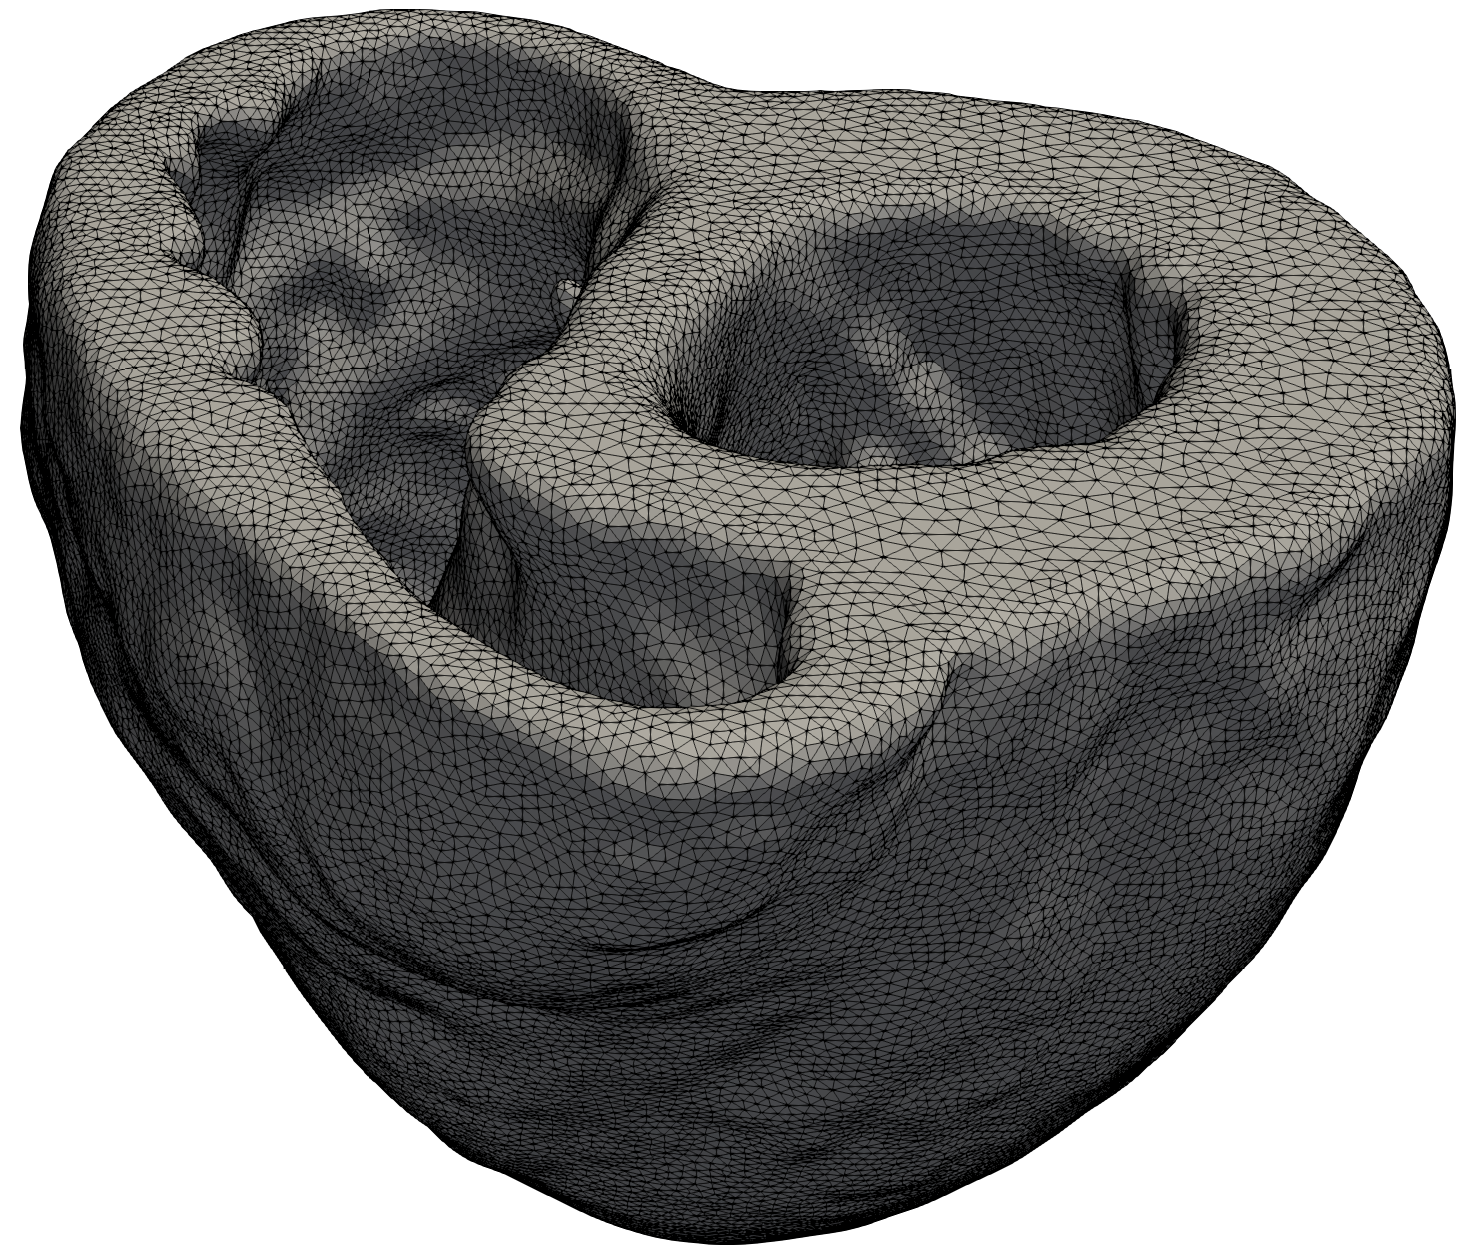
\includegraphics[scale=0.14]{media/4-cardioid/0-ventriclesurf.png}
\label{fig:tet1}}
\subfigure[]{%
		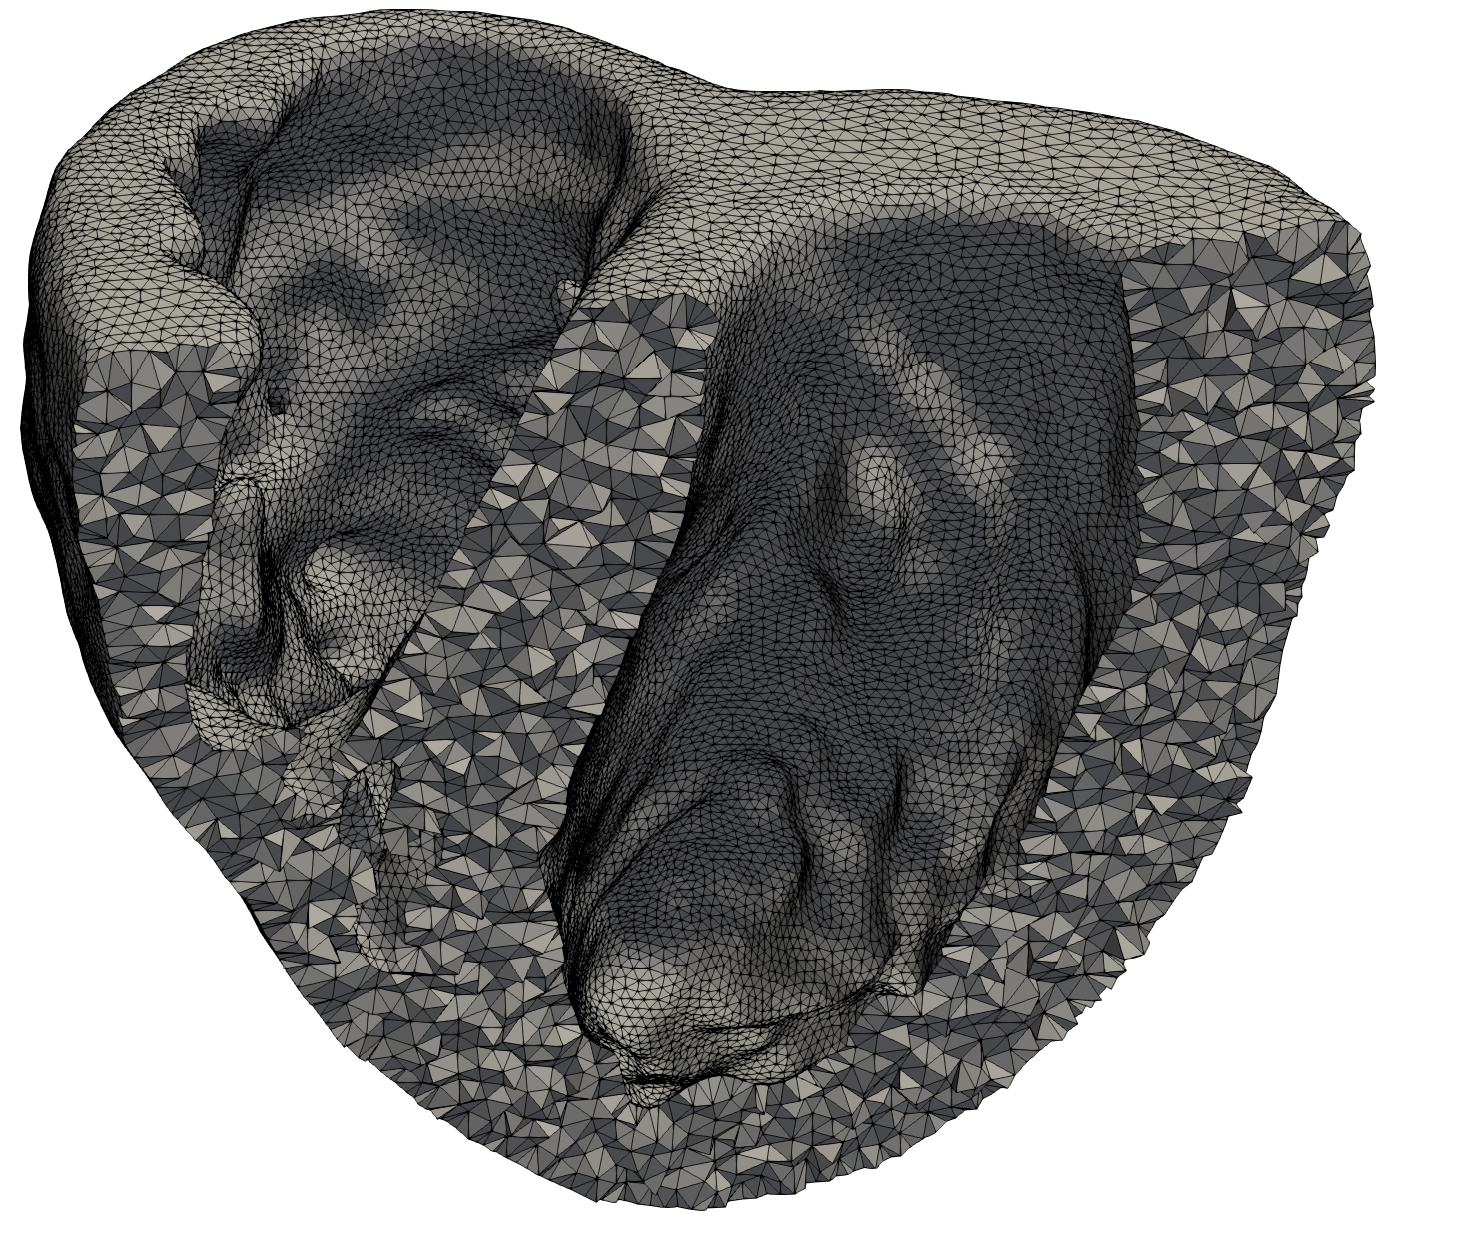
\includegraphics[scale=0.14]{media/4-cardioid/1-tet.png}
\label{fig:tet2}}
%
\caption{Bi-ventricular mesh: (a) surface mesh, and (b) clipped view of quadratic tetrahedral mesh used in Cardioid simulations}
\label{fig:tetmesh}
\end{figure}

\begin{figure}[ht]
\centering
\subfigure[]{%
		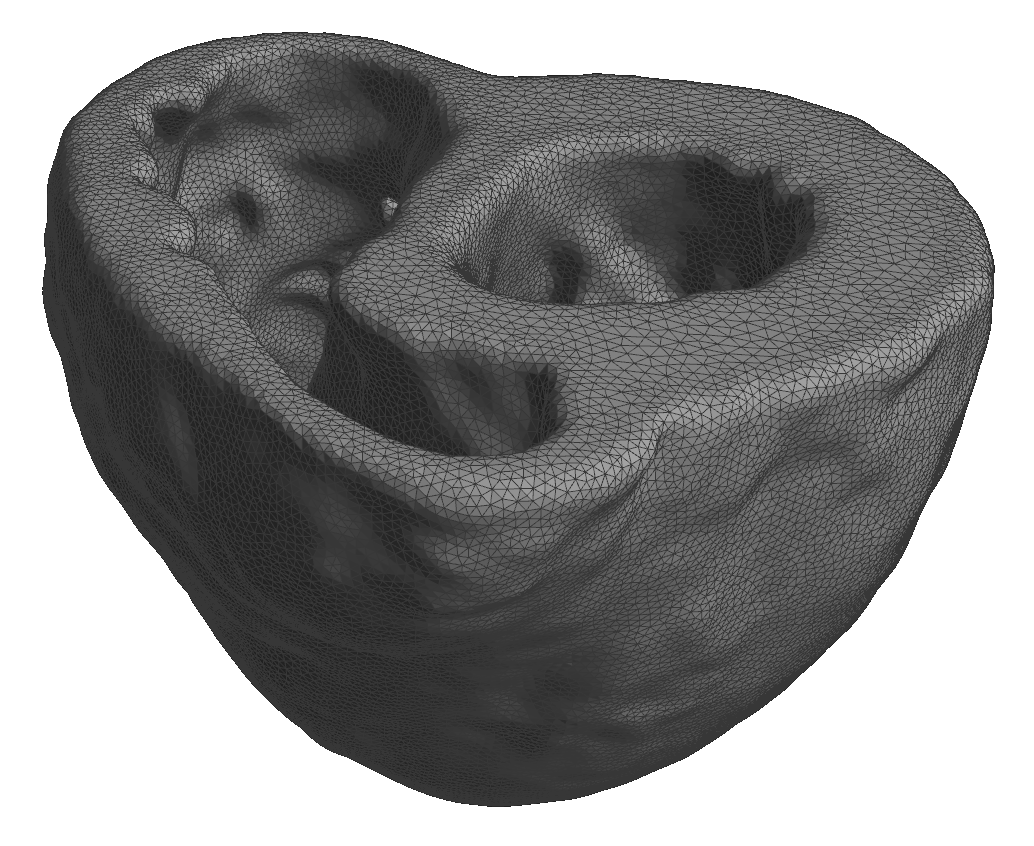
\includegraphics[scale=0.18]{media/3-celeris/1-brep.png}
\label{fig:cel1}}		
\subfigure[]{%
		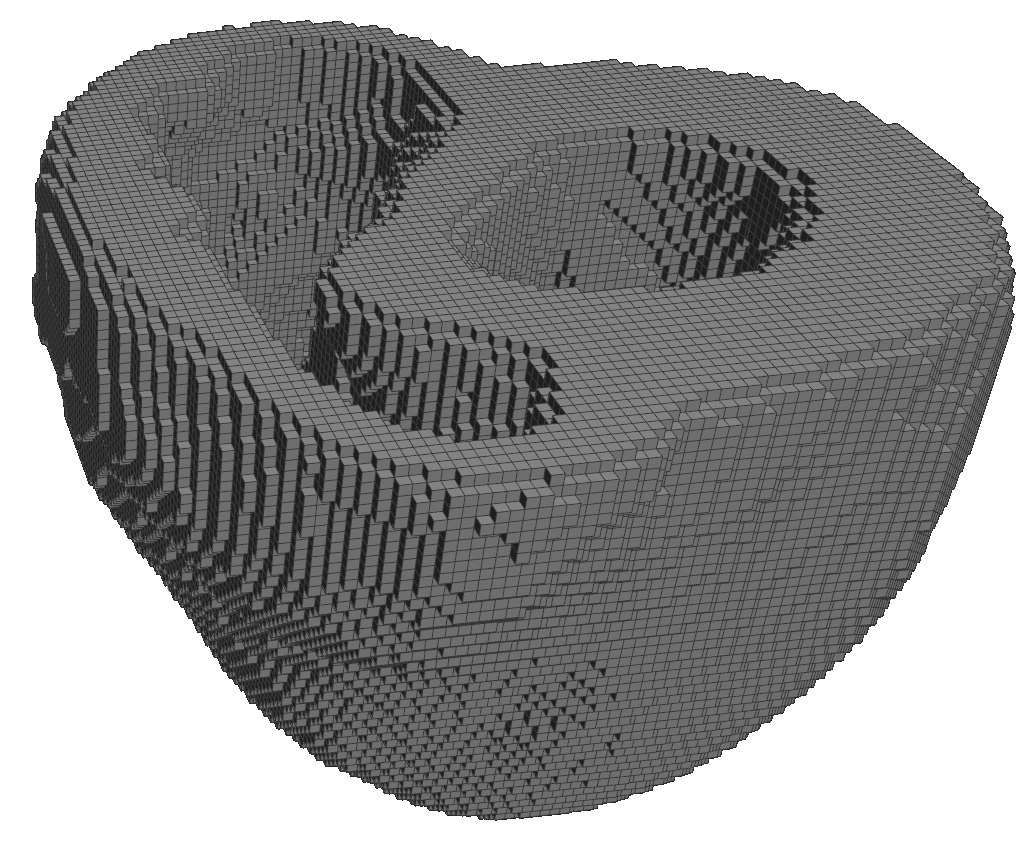
\includegraphics[scale=0.18]{media/3-celeris/2-hex.png}
\label{fig:cel2}}		
\subfigure[]{%
		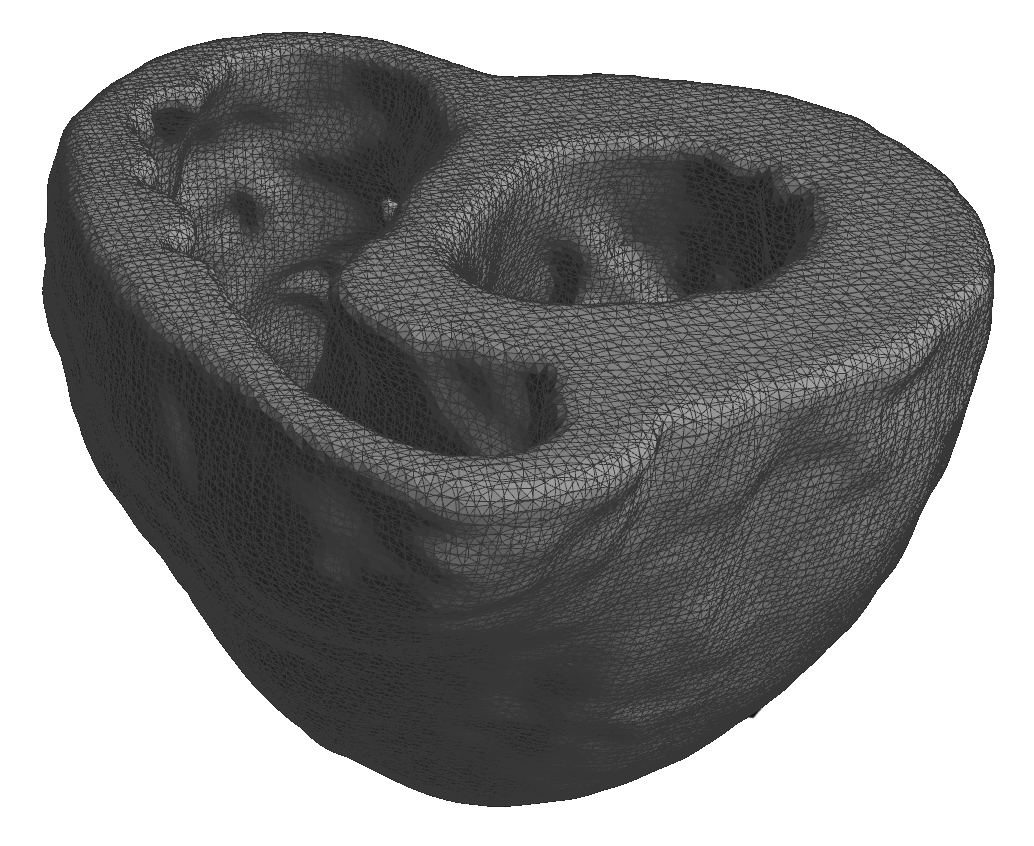
\includegraphics[scale=0.18]{media/3-celeris/3-pmesh.png}
\label{fig:cel3}}		
\subfigure[]{%
		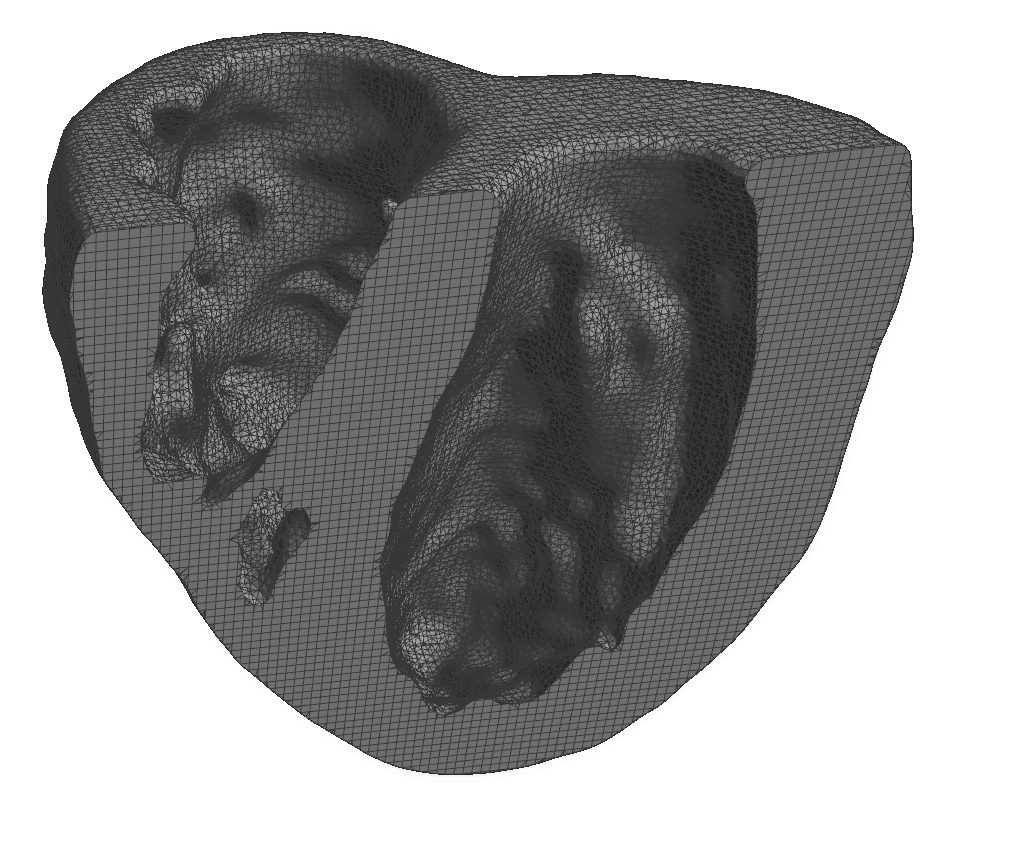
\includegraphics[scale=0.18]{media/3-celeris/4-clip.png}
\label{fig:cel4}}	
\subfigure[]{%
		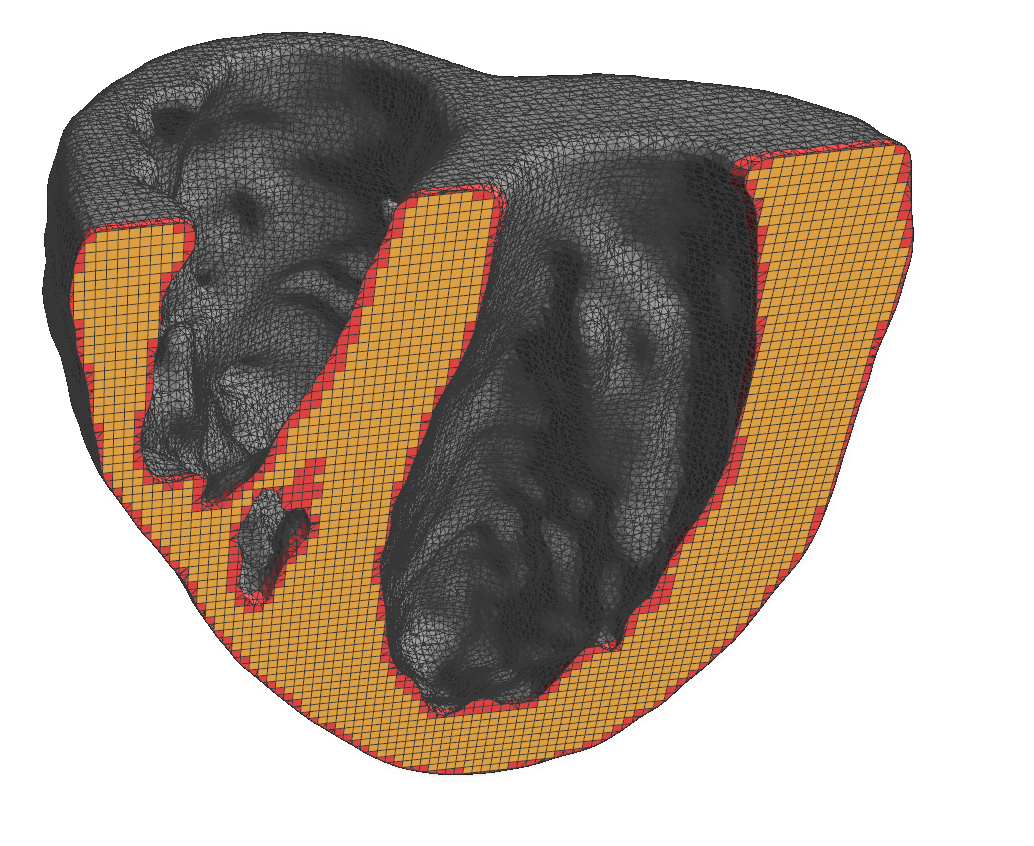
\includegraphics[scale=0.18]{media/3-celeris/5-color.png}
\label{fig:cel5}}			

\caption{Generation of polyhedral mesh: (a) input surface mesh, (b) bounding hex mesh,  (c) resulting polyhedral mesh, (d) clipped mesh, and (e) highlight of elements with cuboidal vs. general polyhedral shape.}
\label{fig:cel}
\end{figure}

\begin{figure}[ht]
\centering
\subfigure[]{%
		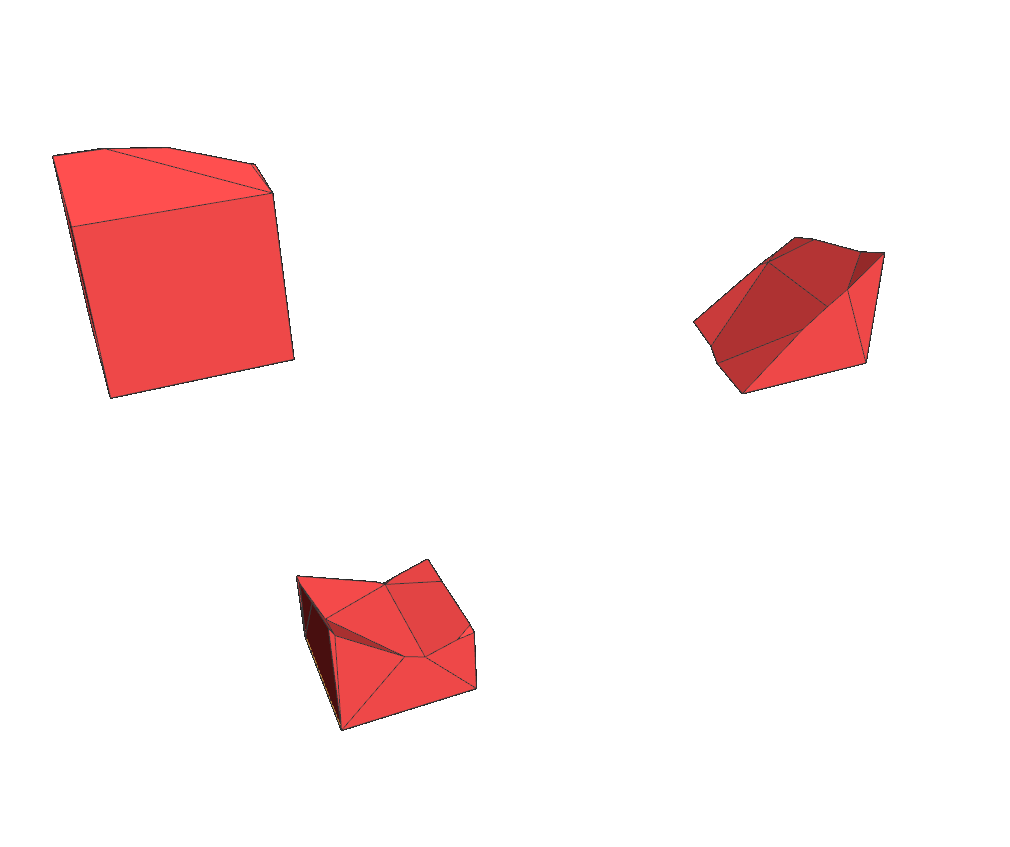
\includegraphics[scale=0.125]{media/3-celeris/zoom/zoom1.png}
\label{fig:zoom1}}		
\subfigure[]{%
		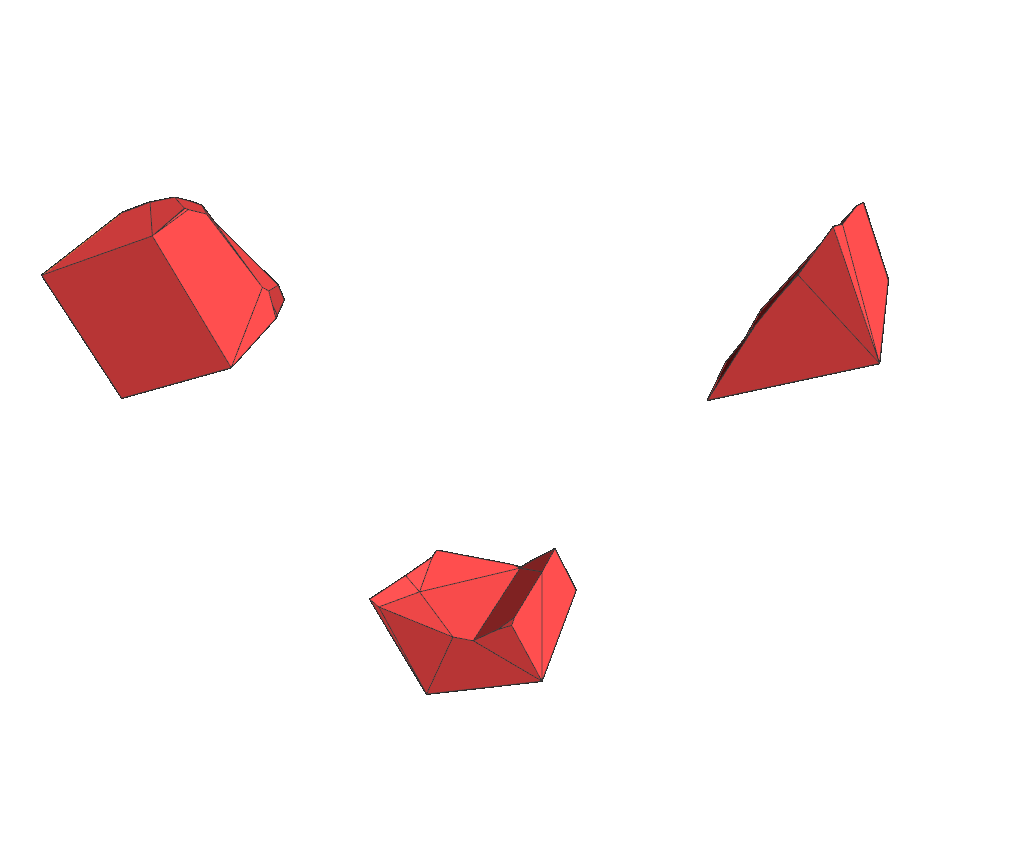
\includegraphics[scale=0.125]{media/3-celeris/zoom/zoom2.png}
\label{fig:zoom2}}		
\subfigure[]{%
		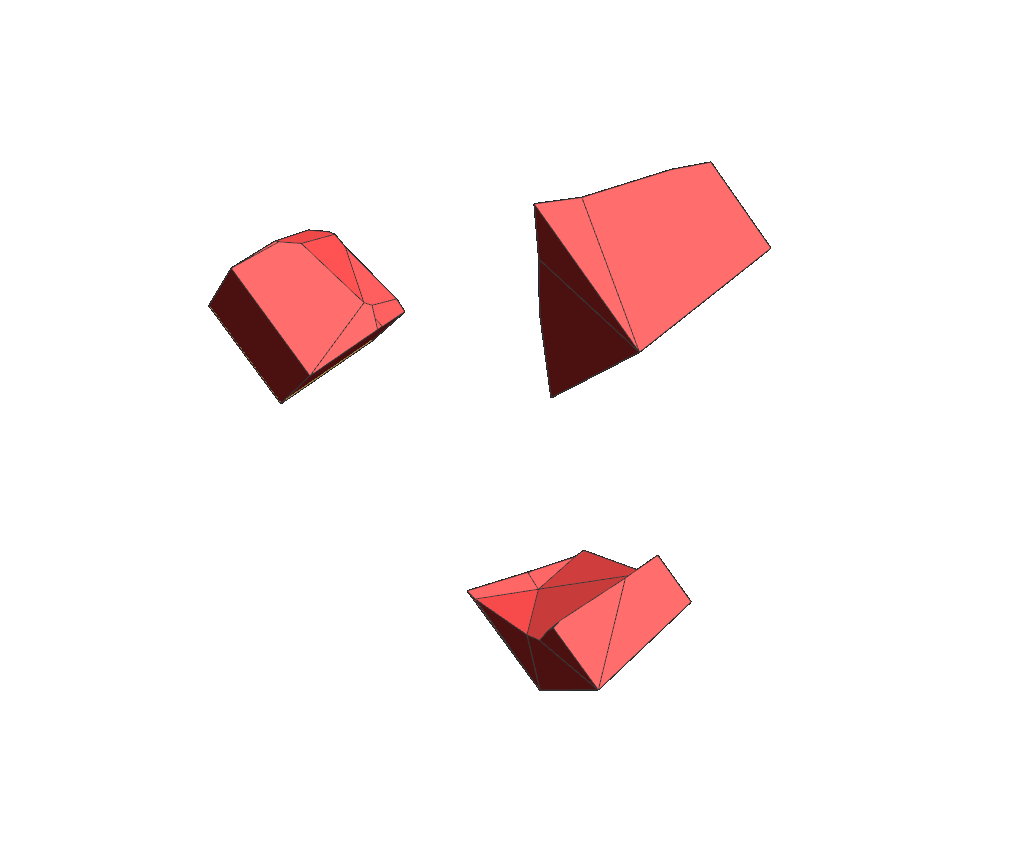
\includegraphics[scale=0.125]{media/3-celeris/zoom/zoom3.png}
\label{fig:zoom3}}		
\subfigure[]{%
		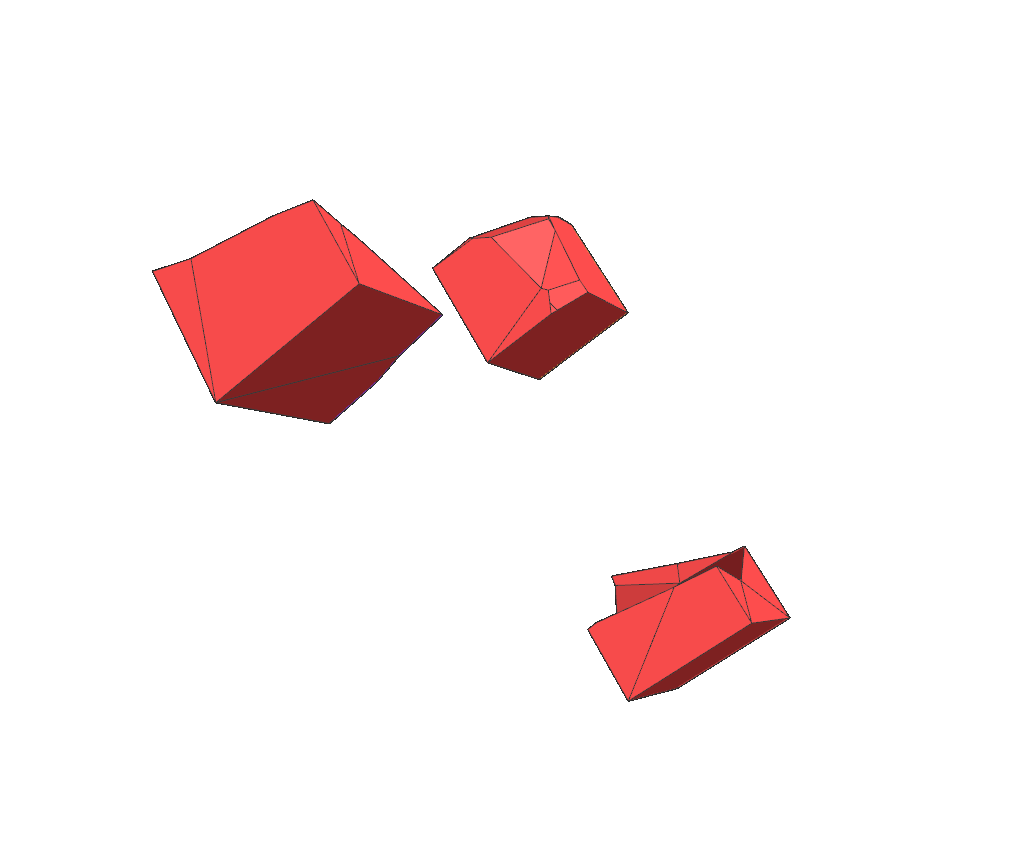
\includegraphics[scale=0.125]{media/3-celeris/zoom/zoom4.png}
\label{fig:zoom4}}	
\subfigure[]{%
		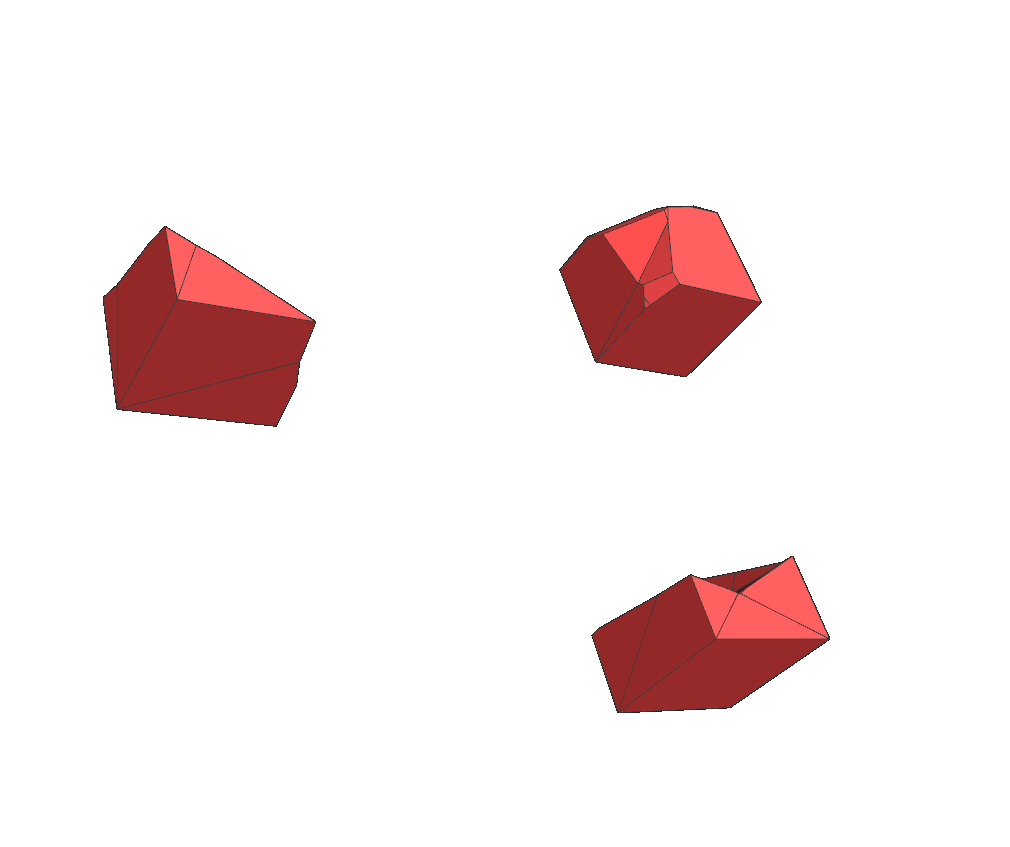
\includegraphics[scale=0.125]{media/3-celeris/zoom/zoom5.png}
\label{fig:zoom5}}		
\subfigure[]{%
		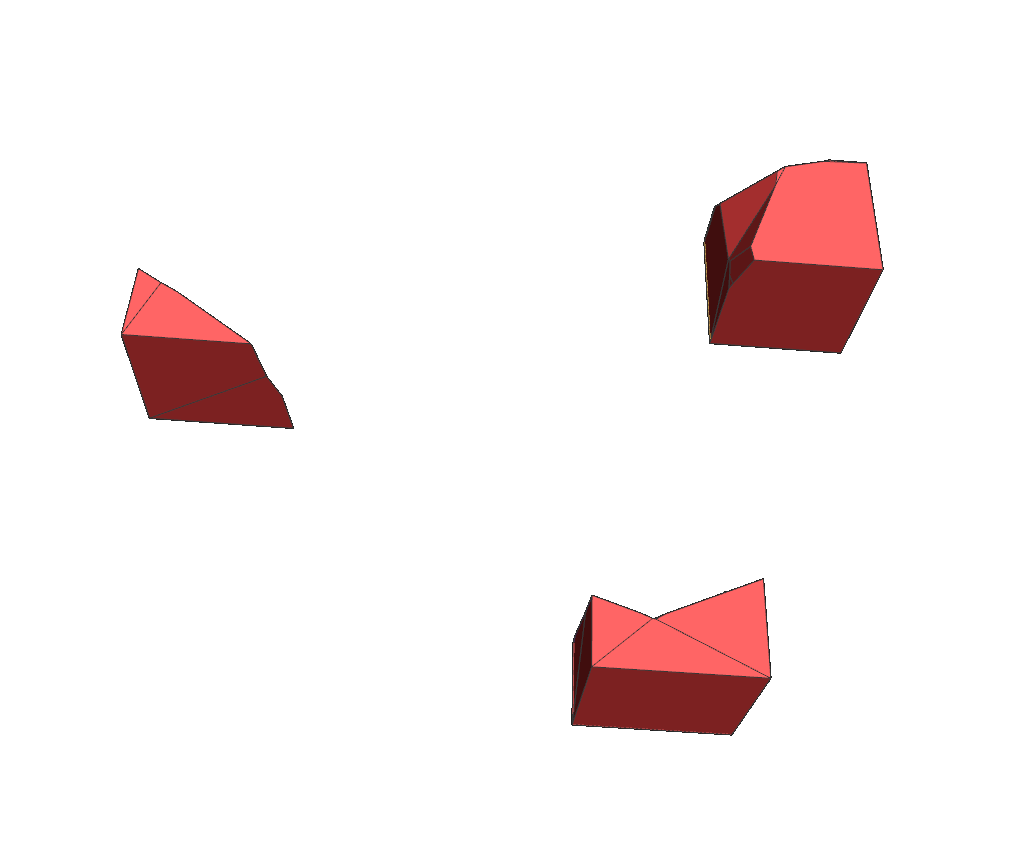
\includegraphics[scale=0.125]{media/3-celeris/zoom/zoom6.png}
\label{fig:zoom6}}	

\caption{Three example arbitrary polyhedral elements presented at different angles}
\label{fig:zoom}
\end{figure}

\begin{figure}[ht]
\centering
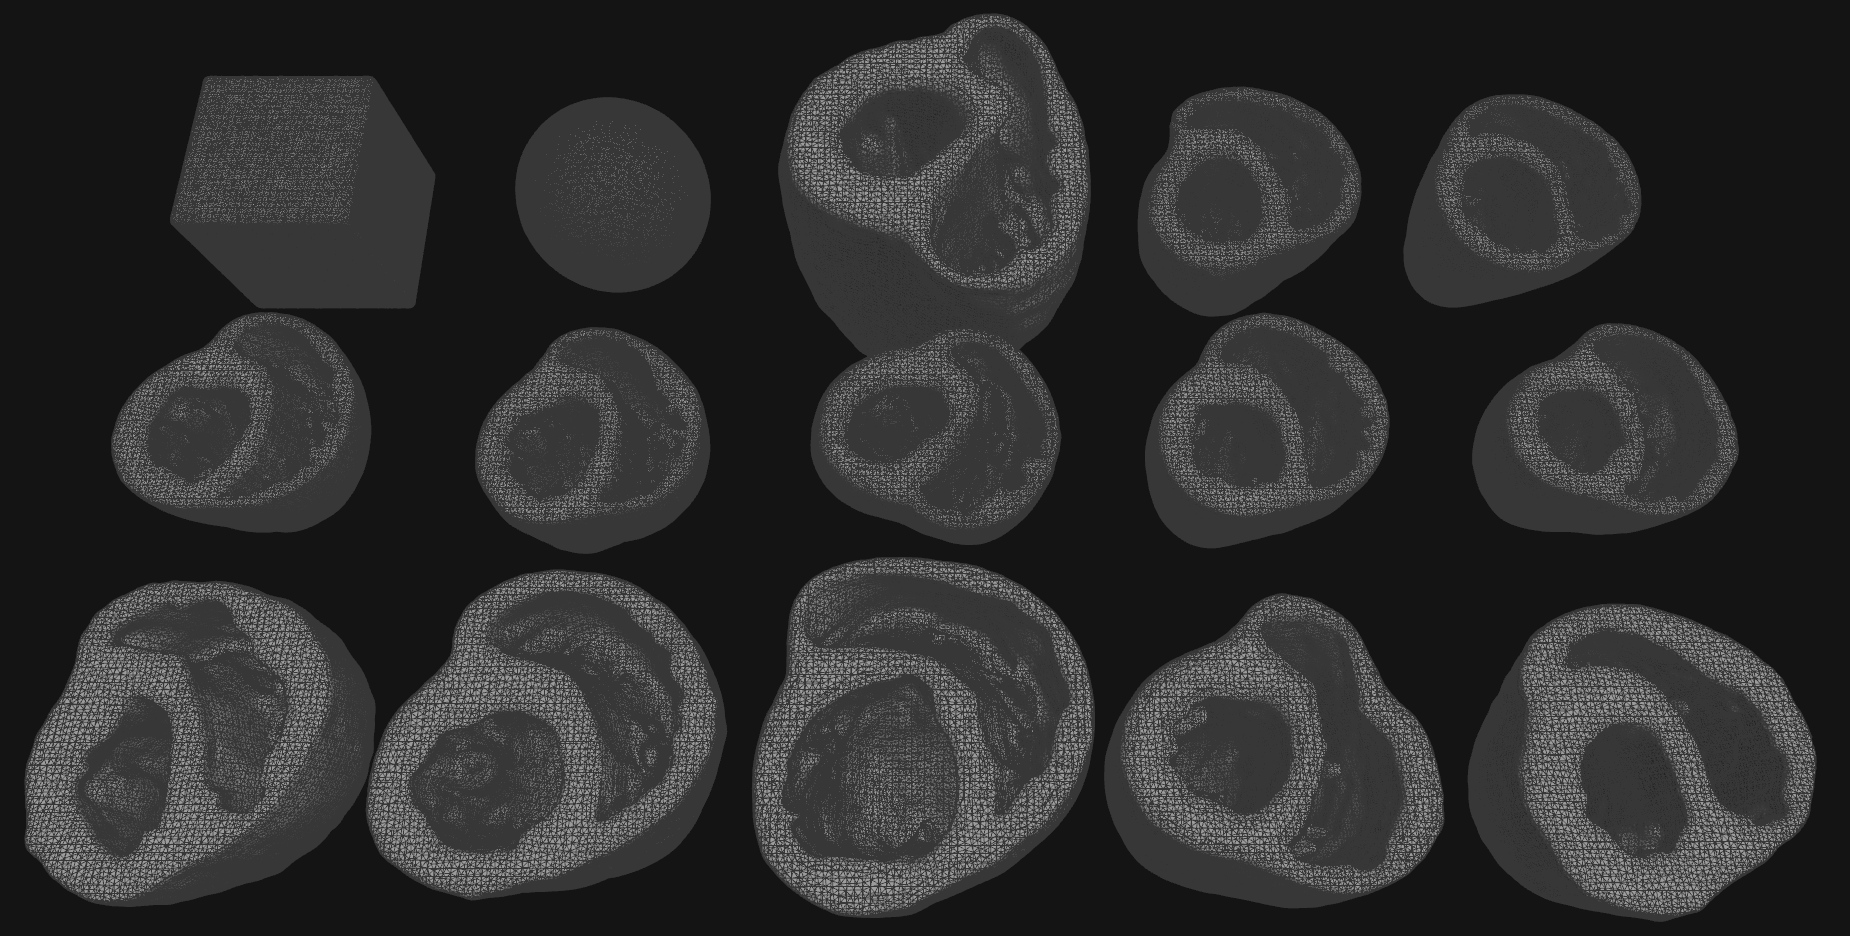
\includegraphics[width=1.0\textwidth]{media/3-celeris/7-suite.png}
\caption{Suite of polyhedral finite element meshes generated from image data \vspace{1cm}}
\label{fig:celsuite}
\end{figure}

%%%%%%%%%%%%%%%%%%%%%%%%%%%%%%%%%%%%%%%%%%%%%%%
%%%%%%%%%%%%%%%%%%%%%%%%%%%%%%%%%%%%%%%%%%%%%%%
\section{File Formats}
\label{File Formats-MESH}